

\tikzset{every picture/.style={line width=0.75pt}} %set default line width to 0.75pt        

\begin{tikzpicture}[x=0.75pt,y=0.75pt,yscale=-1,xscale=1]
%uncomment if require: \path (0,205); %set diagram left start at 0, and has height of 205

%Straight Lines [id:da047694907882628756] 
\draw  [->]  (236,75) -- (396,75) ;
%Straight Lines [id:da7421770675606394] 
\draw  [<-]  (236,115) -- (396,115) ;
%Straight Lines [id:da09790380711372837] 
\draw  [->]  (236,155) -- (396,155) ;
%Straight Lines [id:da8684548711102391] 
\draw  [line width=0.5]  (66,19) -- (174,19) ;
%Straight Lines [id:da6664890562466532] 
\draw  [line width=0.5]  (506,19) -- (534,19) ;

% Text Node
\draw (120,10) node    {$P(( \alpha _{1} ,\dotsc ,\alpha _{n}) ,\phi )$};
% Text Node
\draw (520,10) node    {$V( \phi )$};
% Text Node
\draw (316,111.6) node [anchor=south] [inner sep=0.75pt]    {$c$};
% Text Node
\draw (316,151.6) node [anchor=south] [inner sep=0.75pt]    {$\alpha _{\mathrm{z} 1} ,\dotsc ,\alpha _{\mathrm{z} n} \in \mathbb{Z}_{q}$};
% Text Node
\draw (120,30) node    {$\alpha _{\mathrm{t} j}\overset{\mathrm{R}}{\leftarrow }\mathbb{Z}_{q} \ ( j=1,\dotsc ,n)$};
% Text Node
\draw (520,95) node    {$c\overset{\mathrm{R}}{\leftarrow }\mathcal{C}$};
% Text Node
\draw (120,135) node    {$\alpha _{\mathrm{z} j}\leftarrow \alpha _{\mathrm{t} j} +\alpha _{j} c\ ( j=1,\dotsc ,n)$};
% Text Node
\draw (316,71.6) node [anchor=south] [inner sep=0.75pt]    {$u_{\mathrm{t} 1} ,\dotsc ,u_{\mathrm{t} m} \in \mathbb{G}$};
% Text Node
\draw (120,55) node    {$u_{tj}\leftarrow \prod _{j=1}^{n} g_{ij}^{\alpha _{\mathrm{t} j}} \ ( i=1,\dotsc ,m)$};
% Text Node
\draw (520,175) node    {$\prod _{j=1}^{n} g_{ij}^{\alpha _{\mathrm{z} j}}\overset{?}{=} u_{\mathrm{t} i} \cdot u_{i}^{c} \ ( i=1,\dotsc ,m)$};


\end{tikzpicture}